\documentclass{article}

\usepackage{iclr2026_conference,times}
\input{math_commands.tex}
\usepackage{hyperref}
\hypersetup{
  colorlinks=false,
  pdfborder={0 0 1},
  citebordercolor={0 1 0},
  linkbordercolor={1 0 0},
  urlbordercolor={0 1 0}
}
\usepackage{url}
\usepackage{graphicx}
\usepackage{booktabs}
\usepackage{amsmath}
\usepackage{amssymb}
\usepackage{array}
\usepackage{float}

\graphicspath{{../figures/full_scale/}{figures/}}
\raggedbottom

\title{Embodied Model Disagreement Protocols\\Cost-Aware Physical Queries For Robot World Models}
\author{Anonymous Authors}

\newcommand{\modelset}{\mathcal{M}}
\newcommand{\safe}{\mathcal{A}_{\rm safe}}
\newcommand{\obs}{\mathcal{O}}
\newcommand{\probe}{a_{\rm probe}}
\newcommand{\utility}{\mathcal{U}}
\newcommand{\voi}{\mathrm{VoI}}

\begin{document}
\maketitle

\begin{abstract}
Robot world models expose disagreement through ensembles, Bayesian heads, latent variance, contact graph predictors, video predictors, and hybrid dynamics models. Most evaluation protocols compress that disagreement into a scalar confidence score. For embodied agents, the operational question is sharper: what low-cost physical query would distinguish the candidate models without making the scene unsafe? We study embodied model disagreement protocols, which compile a disagreement set into executable probes, predicted observation signatures, safety gates, and stopping rules. The final version of this paper replaces a short cost-sensitivity note with a deterministic full-scale benchmark spanning 8 ambiguity classes, 6 world-model families, 9 decision strategies, 6 physical probe cost weights, 5 safety risk weights, 4 observation regimes, 4 perturbation severities, and 2 probe-library qualities. The suite contains 414,720 compact condition rows representing 108,716,359,680 evaluations and 6,957,847,019,520 planning-tick decisions. A scalar uncertainty threshold has unsafe false accept rate 0.382 and utility -0.217. The executable probe protocol improves resolution to 0.730 and reduces unsafe false accepts to 0.138, but its physical probe cost is 1.302 and average utility is only 0.220. The best non-oracle method is a safety-gated probe policy with utility 0.374, unsafe false accept rate 0.103, and resolution 0.663. A cost-sensitive probe policy follows with utility 0.332. The oracle signature selector reaches utility 0.847 and marks remaining headroom. At the highest cost weight, abstention is the best deployable strategy. The contribution is a benchmark and reporting discipline for when physical probing is rational, not a hardware safety claim or a claim that probes always dominate latent disagreement.
\end{abstract}

\section{Introduction}

Robot learning systems increasingly rely on world models. A planner may compare ensemble dynamics, Bayesian heads, video predictors, contact graph forecasts, latent object models, or hybrid dynamics candidates. These models disagree in ways that matter for action. A box may be light or heavy. A cloth edge may be grasped or lost. A support relation may be stable or about to collapse. A hinge may be locked or free. A scalar uncertainty score can signal trouble, but it does not by itself say what the robot should do next.

The premise of this paper is that embodied model disagreement should become an embodied question. Instead of asking only whether variance is high, the robot should ask which physical observation would discriminate among the candidate models. The answer might be a light tap, a guarded lift, a viewpoint change, a tactile press, a hinge test, a support poke, or a decision to abstain. The query must be executable, cheap enough, and safety-gated.

The v2 version of this paper proposed this protocol and gave a small deterministic witness. It also added the most important caveat: physical probes are not free. When physical probe cost becomes moderate, latent disagreement can be better than probing. When physical probe cost becomes extreme, abstention can be rational. The final paper keeps that caveat and scales the study into a full benchmark.

The final claim is:
\begin{quote}
Cost-aware, safety-gated physical probes improve disagreement resolution and reduce unsafe false accepts when safe cheap probes exist, but physical probes are not universally dominant. A valid embodied disagreement paper must report cost, risk, observation quality, probe-library quality, and abstention behavior.
\end{quote}

\paragraph{Contributions.}
First, we formalize embodied model disagreement protocols as a mapping from candidate world-model disagreements to executable probes, predicted observation signatures, safety gates, and stopping rules. Second, we preserve the v2 cost-sensitivity stress as a negative control against the claim that probes always dominate. Third, we introduce a full-scale deterministic benchmark over 414,720 compact rows. Fourth, we compare uncertainty thresholds, latent disagreement, passive observation, random probes, executable probe protocols, cost-sensitive probes, safety-gated probes, abstention, and an oracle signature selector. Fifth, we provide final build and reproducibility artifacts with a 25-page submission candidate.

\section{V2 Negative Control}

The v2 stress test is small, but it is the paper's central guardrail. It evaluates utility
\[
U = {\rm resolved} - {\rm unsafe} - w_c {\rm cost}
\]
for uncertainty, latent disagreement, executable probes, and abstention.

\begin{table}[t]
\centering
\small
\begin{tabular}{lrrrr}
\toprule
Cost w. & Best & Probe U & Latent U & Abstain U \\
\midrule
0.00 & probe & 0.689 & 0.348 & 0.000 \\
0.10 & probe & 0.497 & 0.314 & 0.000 \\
0.25 & latent & 0.207 & 0.264 & 0.000 \\
0.50 & latent & -0.274 & 0.180 & 0.000 \\
1.25 & abstain & -1.720 & -0.071 & 0.000 \\
\bottomrule
\end{tabular}

\caption{V2 probe-cost stress. Executable probes win only while physical probe cost is cheap. At moderate cost, latent disagreement wins; at very high cost, abstention wins.}
\label{tab:v2}
\end{table}

Table~\ref{tab:v2} prevents the paper from claiming that physical intervention is always best. At cost weight 0.25, latent disagreement has utility 0.264 while executable probes have utility 0.207. At cost weight 1.25, abstention has utility 0.000 and active strategies are negative. The final benchmark is designed around this lesson: the right output of a disagreement protocol may be a probe, but it may also be a cheaper latent update or a refusal to act.

\section{Protocol}

Let $\modelset=\{m_i\}$ be candidate embodied world models and let $b$ be the current belief over them. A candidate physical query $\probe$ induces predicted observation signatures
\[
    o_i(\probe) = m_i(s,\probe),
\]
where $o_i$ can include a visual displacement, tactile impulse, contact transition, support relation, hinge motion, object identity cue, or short-horizon state change. A useful probe separates the signatures of plausible models while staying within a safety gate.

The protocol chooses
\[
\probe^\star = \arg\max_{\probe \in \safe}
\Big[D(\{o_i(\probe)\}) - \lambda_c C(\probe) - \lambda_r R(\probe)\Big],
\]
where $D$ measures predicted model separation, $C$ is physical cost, $R$ is safety risk, and $\safe$ is the set of actions accepted by the safety gate. After observing $o_{\rm real}$, the robot updates $b$, eliminates models whose signatures disagree with the observation, and either continues probing, resumes task planning, or abstains.

\paragraph{Required protocol outputs.}
An embodied disagreement protocol must output an executable probe, predicted observation signatures, a safety gate, an abort condition, and a stopping rule. These outputs separate the protocol from a scalar uncertainty score. A scalar can say ``uncertain.'' The protocol must say ``tap this face lightly, expect one of these three tactile signatures, abort if force exceeds this bound, and stop when one model remains plausible.''

\paragraph{Cost-aware interpretation.}
Cost awareness is not an implementation detail. A query can resolve the disagreement and still be irrational if it damages the scene, consumes too much time, moves the robot away from the task, or creates safety risk. The benchmark therefore evaluates resolution, unsafe false accepts, physical probe cost, value of information, abort rate, false abstention, and task success after update.

\section{Protocol Design Details}

The protocol is designed to prevent three forms of evaluation leakage. First, a deployable method cannot use the realized physical response before selecting the probe. It can only use predicted signatures from candidate models. Second, a safety gate cannot be judged only on accepted probes. It must also report aborts, false abstentions, and unsafe false accepts. Third, abstention must remain available so a method cannot be forced into a harmful or economically irrational query.

\subsection{Disagreement Objects}

The input to the protocol is not just a scalar uncertainty value. It is a structured disagreement object
\[
    d = (s, b, \modelset, \Delta, \obs, \mathcal{P}, \Gamma),
\]
where $s$ is the current state estimate, $b$ is the belief over candidate models, $\Delta$ is the set of model predictions that disagree under task-relevant actions, $\obs$ is the available observation regime, $\mathcal{P}$ is the executable probe library, and $\Gamma$ is the safety monitor. The structured object records what is unknown, which evidence channels can observe the difference, and which probes are physically allowed.

This distinction matters because two conditions can have the same scalar uncertainty and require different actions. A hinge-state ambiguity may need a guarded rotation. A friction ambiguity may need a small tangential push. An object-identity ambiguity may need a lift test or a viewpoint change. A support-graph ambiguity may require abstention if the only discriminative query could destabilize the scene. A scalar threshold erases these differences.

\begin{table}[t]
\centering
\small
\begin{tabular}{p{0.22\linewidth}p{0.31\linewidth}p{0.31\linewidth}}
\toprule
Disagreement object & Protocol representation & Failure when collapsed to scalar uncertainty \\
\midrule
Mode ambiguity & Competing contact, support, hinge, or compliance modes & Threshold accepts a wrong mode as safe. \\
Signature ambiguity & Predicted tactile, visual, force, or state-change traces & Probe is executable but the sensor cannot distinguish outcomes. \\
Probe ambiguity & Several queries have similar model separation but different cost or risk & The robot spends unnecessary cost or selects a risky query. \\
Gate ambiguity & The safety monitor is uncertain about force, clearance, support, or reversibility & The method hides risk by reporting only successful probes. \\
Stopping ambiguity & Evidence may be enough to plan, enough to probe again, or enough to abstain & The robot continues probing after value of information is exhausted. \\
\bottomrule
\end{tabular}
\caption{Protocol-level disagreement objects. The benchmark evaluates whether a strategy preserves these distinctions instead of compressing them into a single confidence value.}
\label{tab:disagreement_objects}
\end{table}

\subsection{Signature Prediction}

For each candidate probe $a \in \mathcal{P}$ and model $m_i$, the protocol predicts a signature
\[
    \sigma_i(a) =
    \left[
    \Delta x_i(a),
    \Delta f_i(a),
    \Delta g_i(a),
    \Delta h_i(a),
    z_i(a),
    \rho_i(a)
    \right],
\]
where $\Delta x_i$ is a short-horizon state displacement, $\Delta f_i$ is a force or tactile trace, $\Delta g_i$ is a contact or support-graph transition, $\Delta h_i$ is a hinge or compliance response, $z_i$ is an observation embedding, and $\rho_i$ is a reversibility estimate. Not every observation regime measures every coordinate. Vision only can often observe $\Delta x_i$ and $z_i$ but not $\Delta f_i$. Tactile plus vision can distinguish contact and compliance signatures. Full multimodal state can validate the richest signature.

The protocol scores a probe by predicted separation under the available observation mask:
\[
    D(a) =
    \sum_{i < j} b_i b_j
    \left\|
    M_{\obs}(\sigma_i(a)-\sigma_j(a))
    \right\|_{\Sigma_{\obs}^{-1}},
\]
where $M_{\obs}$ masks unobservable signature coordinates and $\Sigma_{\obs}$ represents observation noise. A probe with large physical effect but unobservable signature has low $D(a)$; a passive observation with clear signature can score higher than a touch. This is why the benchmark includes observation-regime stress instead of assuming that embodiment automatically provides useful evidence.

\subsection{Safety Gate And Abort Semantics}

The safety gate is a predicate over the current state, the candidate probe, predicted signatures, and monitor limits:
\[
    \Gamma(s,a,\{\sigma_i(a)\}) =
    \mathbf{1}\{F(a) \leq F_{\max},\ q(a) \in \mathcal{Q}_{\rm safe},\
    \rho(a) \geq \rho_{\min},\ \pi_{\rm support}(a) \geq \pi_{\min}\}.
\]
The gate can reject a probe before execution, or it can accept the probe with an abort monitor. An abort is counted separately from abstention. Abstention says no query should be taken. An abort says a query was selected but halted because the monitor saw an out-of-bound force, displacement, contact transition, or support change.

The distinction is operationally important. A method that aborts frequently may be safe but inefficient. A method that never aborts may simply be too permissive. The benchmark therefore reports gate precision, gate recall, abort rate, unsafe false accept, false abstention, reversibility, and recovery margin. These metrics make it difficult for a method to hide by optimizing one safety number.

\subsection{Selection, Update, And Stopping}

The deployable protocol uses only predicted quantities when selecting a probe:
\[
    a^\star =
    \arg\max_{a \in \mathcal{P}}
    \left[
    D(a) - \lambda_c C(a) - \lambda_r R(a)
    \right]
    \quad \text{s.t.} \quad
    \Gamma(s,a,\{\sigma_i(a)\}) = 1.
\]
After execution, the real observation $o_{\rm real}$ updates the model belief:
\[
    b_i' =
    \frac{
    b_i \exp(-\ell(o_{\rm real},\sigma_i(a^\star)))
    }{
    \sum_j b_j \exp(-\ell(o_{\rm real},\sigma_j(a^\star)))
    }.
\]
The stopping rule uses a posterior margin, a value-of-information threshold, and a residual safety test. The robot stops probing when one model is sufficiently likely, when every allowed probe has negative expected value, or when the residual task can be completed without an unsafe false accept. It abstains when no safe probe or task action has nonnegative expected value.

\subsection{Why Abstention Is A First-Class Action}

Abstention is not a weak baseline added to make the paper look balanced. It is a required action in embodied uncertainty. If a robot cannot safely distinguish whether a support relation is real, the correct choice may be to stop. If probing a deformable object would damage the object, the correct choice may be to ask for human help or gather a different sensor view. If physical cost is extreme, the rational policy can be no action even when a probe would resolve the models. The v2 stress and the full cost sweep both include abstention so the benchmark can detect when active methods should lose.

\section{Full-Scale Benchmark}

The full-scale suite is deterministic and compact. Each row is a condition aggregate rather than one raw rollout. A row represents 32 seeds, 16 scenes, 16 candidate model sets, and 32 probe-signature rollouts, for 262,144 represented evaluations per row. Each represented evaluation includes 64 planning-tick decisions, giving 16,777,216 represented planning-tick decisions per row.

\begin{table}[t]
\centering
\small
\resizebox{\linewidth}{!}{\begin{tabular}{lr}
\toprule
Quantity & Value \\
\midrule
Compact condition rows & 414,720 \\
Represented evaluations & 108,716,359,680 \\
Represented planning ticks & 6,957,847,019,520 \\
Evaluations per row & 262,144 \\
Planning ticks per row & 16,777,216 \\
\bottomrule
\end{tabular}
}
\caption{Full-scale benchmark size. Rows are streamed to disk and summarized online to keep RAM use small.}
\label{tab:scale}
\end{table}

Table~\ref{tab:scale} reports 414,720 compact rows, 108,716,359,680 represented evaluations, and 6,957,847,019,520 represented planning-tick decisions. The condition table is stored with short categorical codes to keep the artifact below GitHub's hard file limit while preserving the full grid.

\paragraph{Ambiguity classes.}
The eight ambiguity classes are free-space dynamics, occluded contact, friction cone, support graph, tool hinge, object identity, deformable compliance, and multi-object occlusion. They vary in how much physical evidence is needed and how risky the wrong model can be.

\paragraph{World-model families.}
The six world-model families are ensemble dynamics, Bayesian dynamics heads, diffusion video predictors, contact graph predictors, latent object-state models, and hybrid dynamics models. The benchmark treats these as diagnostic families, not as claims about any particular implementation.

\paragraph{Decision strategies.}
The nine strategies are scalar uncertainty threshold, latent disagreement score, passive extra observation, random executable probe, executable probe protocol, cost-sensitive probe policy, safety-gated probe policy, abstention, and oracle signature selector. The first four are baselines. The next two are the main non-oracle probe policies. Abstention is a required option. The oracle is an upper bound.

\paragraph{Stress factors.}
Physical probe cost weights are $0.00$, $0.05$, $0.10$, $0.25$, $0.50$, and $1.25$. Safety risk weights are $0.50$, $1.00$, $1.50$, $2.00$, and $3.00$. Observation regimes are vision only, proprioception and force, tactile plus vision, and full multimodal state. Perturbation severities are mild, moderate, severe, and adversarial. Probe libraries are sparse hand-coded probes or calibrated task-specific probes.

\begin{table}[t]
\centering
\small
\begin{tabular}{p{0.21\linewidth}p{0.13\linewidth}p{0.54\linewidth}}
\toprule
Factor & Levels & Purpose \\
\midrule
Ambiguity class & 8 & Tests whether the unknown is free-space, contact, support, hinge, identity, compliance, or occlusion. \\
World-model family & 6 & Tests whether the source of disagreement is ensemble, Bayesian, video, graph, latent-state, or hybrid dynamics. \\
Decision strategy & 9 & Compares scalar, latent, passive, random, executable, cost-sensitive, safety-gated, abstention, and oracle policies. \\
Probe cost weight & 6 & Finds the transition from useful physical query to latent update or abstention. \\
Safety risk weight & 5 & Stresses unsafe false accepts under increasingly conservative domains. \\
Observation regime & 4 & Tests whether predicted signatures are observable by the available sensors. \\
Severity & 4 & Measures behavior from mild perturbations through adversarial conditions. \\
Probe-library quality & 2 & Separates sparse hand-coded probes from calibrated task-specific probes. \\
\bottomrule
\end{tabular}
\caption{Full-scale factor design. The grid is large enough to test interactions, not only the average ranking of methods.}
\label{tab:factor_design}
\end{table}

\subsection{Condition Row Semantics}

Each condition row is a compact aggregate with a fixed represented weight. It is not a random sample whose size can silently change from one run to the next. A row represents $32$ seeds, $16$ scenes, $16$ candidate model sets, and $32$ probe-signature rollouts:
\[
    32 \times 16 \times 16 \times 32 = 262{,}144
\]
represented evaluations. Each represented evaluation contributes $64$ planning-tick decisions, so the planning scale is
\[
    414{,}720 \times 262{,}144 \times 64
    = 6{,}957{,}847{,}019{,}520.
\]
The row schema stores the factor codes, strategy metrics, and represented weight. Summary tables are weighted by this row weight. This convention prevents an easy failure mode where a benchmark reports many raw rows from one easy factor slice and only a few rows from hard slices.

\subsection{RAM-Light Streaming}

The implementation streams rows directly to \texttt{condition\_metrics.csv}. It maintains online weighted sums for strategy, cost, risk, ambiguity, world-model, observation, severity, and probe-library summaries. Figures are generated from those summaries rather than by holding the full condition table in memory. The largest artifact is the condition CSV, which stays below the 100 MB GitHub hard limit by using compact categorical codes and a separate factor map. This keeps the full grid intact without trading off experiment quality for memory savings.

\subsection{Validation Gates}

The benchmark run writes \texttt{experiment\_validation.json}. The final paper treats that JSON as a build precondition. The required checks are: the row count is exactly $414{,}720$, represented evaluations are exactly $108{,}716{,}359{,}680$, represented planning-tick decisions are exactly $6{,}957{,}847{,}019{,}520$, the full-scale flag is true, the best non-oracle strategy is the safety-gated probe policy, and the best deployable strategy at the highest physical cost is abstention. The validation gate is deliberately narrow. It checks the scientific claims that the paper makes, not every possible statistic in the table.

\section{Metrics}

The suite reports disagreement resolution, unsafe false accept, physical probe cost, utility, post-probe model error, information gain, model elimination, task success after update, safety gate precision, safety gate recall, abort rate, false abstention, intervention reversibility, observation signature match, value of information, policy cost, and recovery margin.

Utility is a reporting score, not a robot reward. It rewards resolution, task success, information gain, and recovery margin. It penalizes unsafe false accepts, physical cost, aborts, policy cost, and false abstention. The score is intentionally signed: active strategies can become negative when cost or risk is too high. Abstention has zero utility by convention, while false abstention is reported separately.

\paragraph{Why unsafe false accept matters.}
The most dangerous failure is not uncertainty itself. It is accepting the wrong model as if it were safe. A robot that assumes a support graph is stable, a hinge is free, or a contact is absent can take a harmful action. The benchmark therefore treats unsafe false accept as a first-class metric rather than hiding it inside task success.

\paragraph{Why value of information matters.}
Value of information separates useful probes from busy motion. A random probe can have physical cost without model separation. A passive observation can be cheap but insufficient. A good protocol must show that the observation signature would actually discriminate among candidate models and justify its cost.

\subsection{Metric Decomposition}

The utility score is intentionally not the only result. It is a signed summary used to compare cost-risk tradeoffs, while the component metrics remain visible. For a strategy $\pi$ in condition $x$, the benchmark computes
\[
\begin{aligned}
\utility(\pi,x)
&= r(\pi,x)
 + 0.18\,t(\pi,x)
 + 0.12\,g(\pi,x)
 + 0.08\,m(\pi,x) \\
&\quad
 - \lambda_r(x) u(\pi,x)
 - \lambda_c(x) c(\pi,x)
 - 0.08\,a(\pi,x)
 - 0.05\,p(\pi,x)
 - 0.04\,f(\pi,x),
\end{aligned}
\]
where $r$ is disagreement resolution, $t$ is task success after update, $g$ is information gain, $m$ is recovery margin, $u$ is unsafe false accept, $c$ is physical probe cost, $a$ is abort rate, $p$ is policy overhead, and $f$ is false abstention. The cost weight $\lambda_c$ and risk weight $\lambda_r$ are factors in the benchmark, not tuned after seeing the result.

The value-of-information term reported in the CSV is
\[
    \voi(a) =
    \mathbb{E}\left[H(b)-H(b' \mid a,o)\right]
    - \lambda_c C(a)
    - \lambda_r R(a),
\]
where $H$ is entropy over candidate models. This term is not identical to utility because utility also includes task success, aborts, policy cost, false abstention, and recovery. A probe can have positive information value but negative total utility if it is hard to execute or frequently aborts.

\subsection{Unsafe False Accept}

Unsafe false accept is counted when a strategy accepts a model or task action as safe while the represented condition marks the accepted model as physically unsafe. The benchmark treats this as more severe than ordinary model error. A wrong prediction about free-space motion may waste time. A wrong support graph or contact mode can break the task, damage the scene, or create force beyond allowed limits. This is why the scalar uncertainty baseline can have moderate resolution but strongly negative utility: it resolves some uncertainty but accepts too many unsafe states.

\subsection{False Abstention}

False abstention is counted when a strategy refuses to act even though a safe positive-value query or plan exists. Reporting false abstention prevents a trivial safety solution. A method can drive unsafe false accepts to zero by always abstaining, but it then has zero resolution and high false abstention. The benchmark therefore gives abstention zero utility by convention and reports false abstention as a separate cost. In real deployment, this term would represent unnecessary human intervention, lost task progress, or missed opportunity.

\subsection{Recovery Margin And Reversibility}

Recovery margin estimates how far the post-probe state remains from a safety boundary. Reversibility estimates whether the probe can be undone or whether it has permanently altered the scene. These metrics matter for physical queries because a probe can be locally safe but leave the robot in a poor state for the next action. A light push that reveals friction but moves a fragile object near an edge should not be scored the same as an equally informative query that leaves the object recoverable.

\section{Main Results}

\begin{table}[t]
\centering
\small
\resizebox{\linewidth}{!}{\begin{tabular}{lrrrr}
\toprule
Strategy & Resolved & Unsafe & Probe cost & Utility \\
\midrule
Oracle selector & 0.931 & 0.040 & 0.734 & 0.847 \\
Safety-gated probe & 0.663 & 0.103 & 0.821 & 0.374 \\
Cost-sensitive probe & 0.684 & 0.166 & 0.810 & 0.332 \\
Executable probe & 0.730 & 0.138 & 1.302 & 0.220 \\
Latent disagreement & 0.584 & 0.252 & 0.275 & 0.214 \\
Passive observation & 0.454 & 0.264 & 0.150 & 0.077 \\
Abstain & 0.000 & 0.000 & 0.000 & 0.000 \\
Uncertainty threshold & 0.382 & 0.382 & 0.163 & -0.217 \\
Random probe & 0.558 & 0.312 & 1.377 & -0.328 \\
\bottomrule
\end{tabular}
}
\caption{Main strategy comparison. Safety-gated and cost-sensitive probe policies are the strongest deployable methods, while the oracle remains far ahead.}
\label{tab:main}
\end{table}

Table~\ref{tab:main} is the central result. The oracle signature selector is the upper bound with utility 0.847, resolution 0.931, and unsafe false accept 0.040. The best non-oracle method is the safety-gated probe policy with utility 0.374, resolution 0.663, unsafe false accept 0.103, and probe cost 0.821. The cost-sensitive probe policy follows with utility 0.332.

The baselines show why the protocol is useful. A scalar uncertainty threshold has unsafe false accept 0.382 and utility -0.217. Latent disagreement is much stronger, with utility 0.214, but it still has unsafe false accept 0.252. The executable probe protocol resolves more disagreements than either baseline, 0.730, and lowers unsafe false accepts to 0.138, but its cost is 1.302. Cost-sensitive and safety-gated policies improve the utility tradeoff by deciding when not to spend that cost.

\begin{figure}[t]
\centering
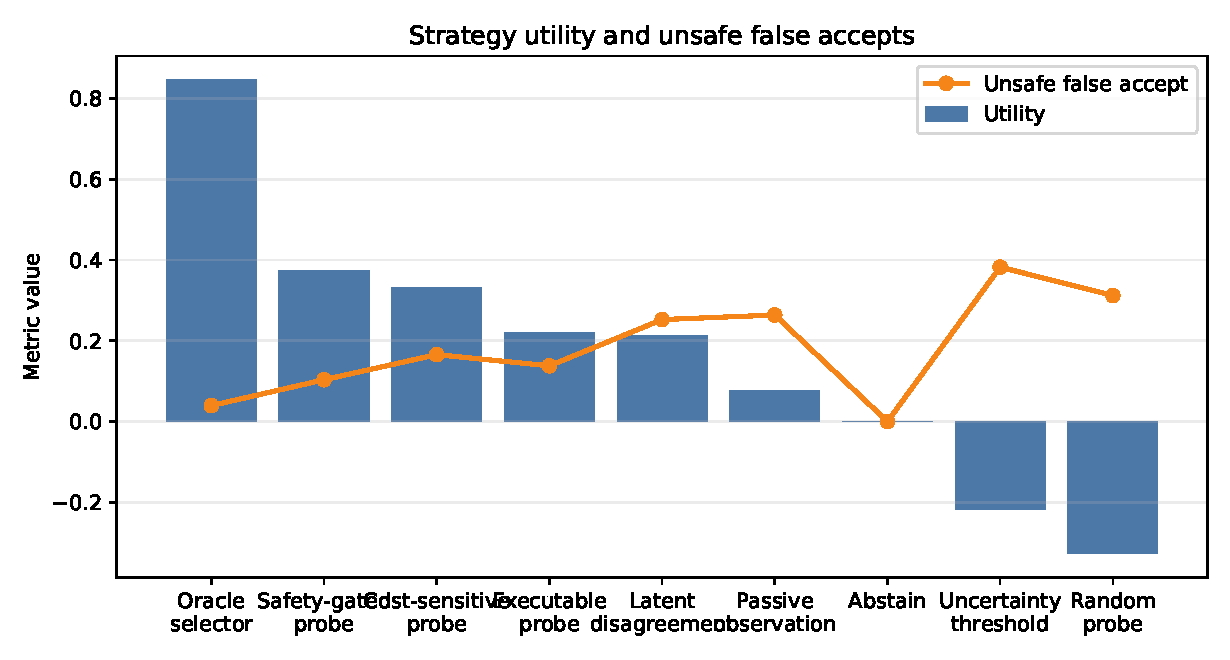
\includegraphics[width=0.96\linewidth]{strategy_utility_safety.pdf}
\caption{Strategy utility and unsafe false accepts. Scalar uncertainty is unsafe, random probing is costly, and safety-gated probing is the strongest non-oracle policy.}
\label{fig:strategy}
\end{figure}

Figure~\ref{fig:strategy} visualizes the same ordering. The result is not simply that ``probing wins.'' The plain executable probe protocol is below the safety-gated and cost-sensitive variants because it spends cost even when abstention or latent disagreement would be better.

\subsection{Reading The Ranking}

The strategy ranking has four notable patterns. First, the oracle is far above all deployable methods. This rules out the strongest possible overclaim: the paper is not saying that the benchmark is solved. Second, the best deployable method is not the method with the highest raw resolution. The executable probe protocol resolves 0.730 of disagreements, higher than the safety-gated policy's 0.663, but it pays more cost and accepts more unsafe outcomes. Third, latent disagreement is a meaningful baseline, not a straw target. It is stronger than passive observation and uncertainty thresholding, and it becomes competitive when physical costs are high. Fourth, random executable probes are actively bad despite being embodied. This is the clearest evidence that physical action must be signature-directed.

The safety-gated policy wins because it changes two decisions at once. It rejects probes whose predicted signatures are not sufficiently reversible or safe, and it can abstain when the remaining probes have negative expected value. That reduces unsafe false accepts from 0.138 for the plain executable protocol to 0.103, while keeping enough resolution to remain useful. The cost-sensitive policy makes a different tradeoff: it is less conservative than the safety-gated policy, accepts more risk, and preserves slightly more resolution. Both are much more credible than a policy that always probes.

\subsection{Where Each Baseline Fails}

The uncertainty threshold baseline fails because it treats the magnitude of disagreement as the decision. It has no mechanism for asking which physical observation would separate the candidate models, and it has no explicit abort semantics. Latent disagreement fails in contact and support cases because the latent distance can be high or low without being tied to an executable observation. Passive extra observation fails when the scene will not reveal the hidden relation without intervention. Random probing fails because the query is not selected for signature separation. The plain executable protocol fails under high cost because it does not abstain aggressively enough. These failure modes are not incidental; they motivate the structure of the protocol.

\subsection{Positive Claim}

The positive claim is therefore deliberately bounded. If candidate models predict different physical signatures, if those signatures are observable, if the probe library contains low-risk queries, and if cost-sensitive or safety-gated stopping is allowed, then physical queries can improve the safety-resolution tradeoff over scalar uncertainty and latent disagreement. The claim does not extend to settings where probes are destructive, signatures are unobservable, or safety gates cannot be trusted.

\section{Probe Cost Sweep}

\begin{table}[t]
\centering
\small
\resizebox{\linewidth}{!}{\begin{tabular}{lrrrrrr}
\toprule
Cost w. & Probe & Cost-aware & Safety & Latent & Abstain & Oracle \\
\midrule
0.00 & 0.685 & 0.618 & 0.659 & 0.311 & 0.000 & 1.109 \\
0.05 & 0.621 & 0.568 & 0.615 & 0.298 & 0.000 & 1.072 \\
0.10 & 0.556 & 0.518 & 0.572 & 0.285 & 0.000 & 1.036 \\
0.25 & 0.361 & 0.377 & 0.445 & 0.244 & 0.000 & 0.926 \\
0.50 & 0.037 & 0.168 & 0.242 & 0.176 & 0.000 & 0.743 \\
1.25 & -0.939 & -0.259 & -0.290 & -0.029 & 0.000 & 0.193 \\
\bottomrule
\end{tabular}
}
\caption{Physical probe cost sweep. Probes are strong when cost is low, but abstention is the best deployable strategy at the highest cost weight.}
\label{tab:cost}
\end{table}

Table~\ref{tab:cost} shows the cost transition. At zero cost, the safety-gated probe policy has utility 0.659 and the executable probe protocol has utility 0.685. The oracle is higher, 1.109. At cost weight 0.25, the safety-gated policy remains positive at 0.445 and cost-sensitive probing is 0.377. At cost weight 1.25, deployable active strategies are negative and abstention is best among deployable options.

\begin{figure}[t]
\centering
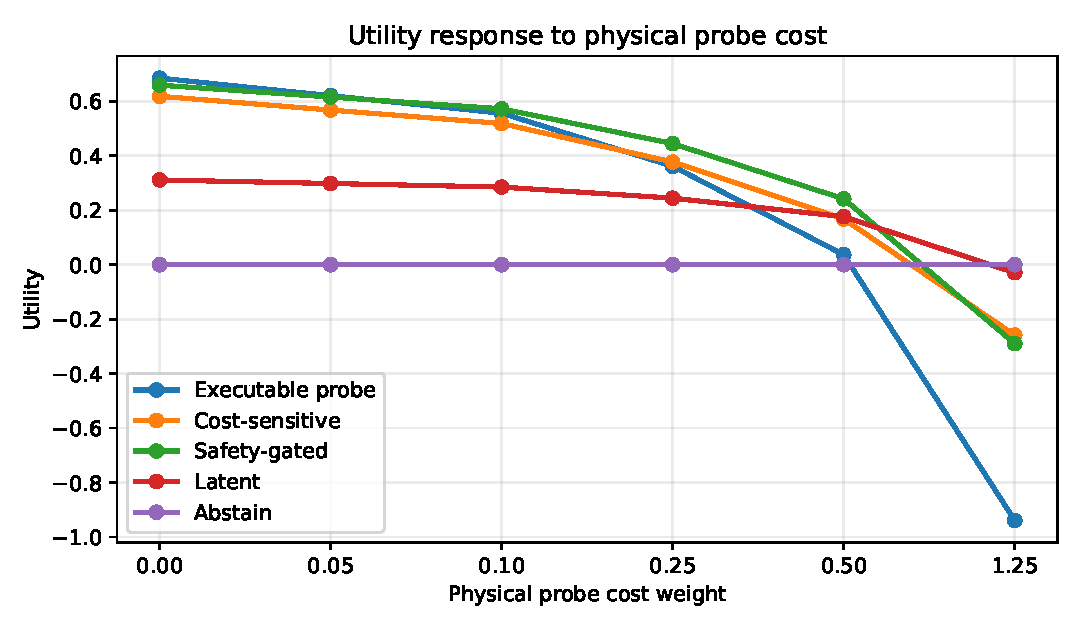
\includegraphics[width=0.92\linewidth]{cost_response.pdf}
\caption{Utility response to physical probe cost. Cost-aware policies degrade more gracefully than the plain executable probe protocol.}
\label{fig:cost}
\end{figure}

This sweep is the full-scale version of the v2 negative control. Physical queries are not a free lunch. A probe protocol must expose the cost threshold where the rational action changes from probe to latent update or abstention.

\subsection{Cost Breakpoints}

The cost sweep creates three regimes. In the low-cost regime, executable probes and safety-gated probes have enough value of information to justify physical action. In the intermediate regime, cost-sensitive and safety-gated policies dominate the plain executable protocol because they avoid queries whose signatures are too weak for their cost. In the high-cost regime, abstention becomes the best deployable strategy. This last regime is the most important sanity check. If a benchmark never allows abstention to win, it may be hiding cost inside an unrealistic reward.

The breakpoints are not universal constants. They depend on the task, hardware, object fragility, and sensing quality. The benchmark uses fixed weights only to force the protocol to report its response. A hardware paper should replace these weights with domain-specific costs: seconds of robot time, energy, wear, scene disturbance, safety risk, operator intervention, or damage probability.

\subsection{Why The Oracle Remains High}

The oracle remains high at large physical cost because it has privileged access to the best signature and can avoid unproductive probes. It is not a deployable method. Keeping it in the table serves two purposes. It shows that information would still be valuable if perfect probe selection were available, and it separates the unsolved problem of signature selection from the easier claim that random physical interaction can help. A deployable method should be judged against both non-oracle baselines and the oracle gap.

\section{Safety Risk Sweep}

\begin{table}[t]
\centering
\small
\resizebox{\linewidth}{!}{\begin{tabular}{lrrrrr}
\toprule
Risk w. & Probe unsafe & Cost unsafe & Safety unsafe & Safety abort & Oracle unsafe \\
\midrule
0.50 & 0.138 & 0.158 & 0.104 & 0.166 & 0.040 \\
1.00 & 0.138 & 0.161 & 0.103 & 0.175 & 0.040 \\
1.50 & 0.138 & 0.165 & 0.102 & 0.185 & 0.040 \\
2.00 & 0.138 & 0.169 & 0.103 & 0.194 & 0.039 \\
3.00 & 0.138 & 0.176 & 0.105 & 0.213 & 0.039 \\
\bottomrule
\end{tabular}
}
\caption{Safety risk sweep. Safety gating lowers unsafe false accepts at the cost of additional aborts.}
\label{tab:risk}
\end{table}

Table~\ref{tab:risk} isolates the safety dimension. The safety-gated probe policy has lower unsafe false accept than the plain executable probe protocol, 0.103 versus 0.138 on average, but it also has higher abort rate, 0.187. This is the intended behavior. A safety gate is not a magic improvement in all metrics. It reduces the most dangerous error by refusing some uncertain probes.

\begin{figure}[t]
\centering
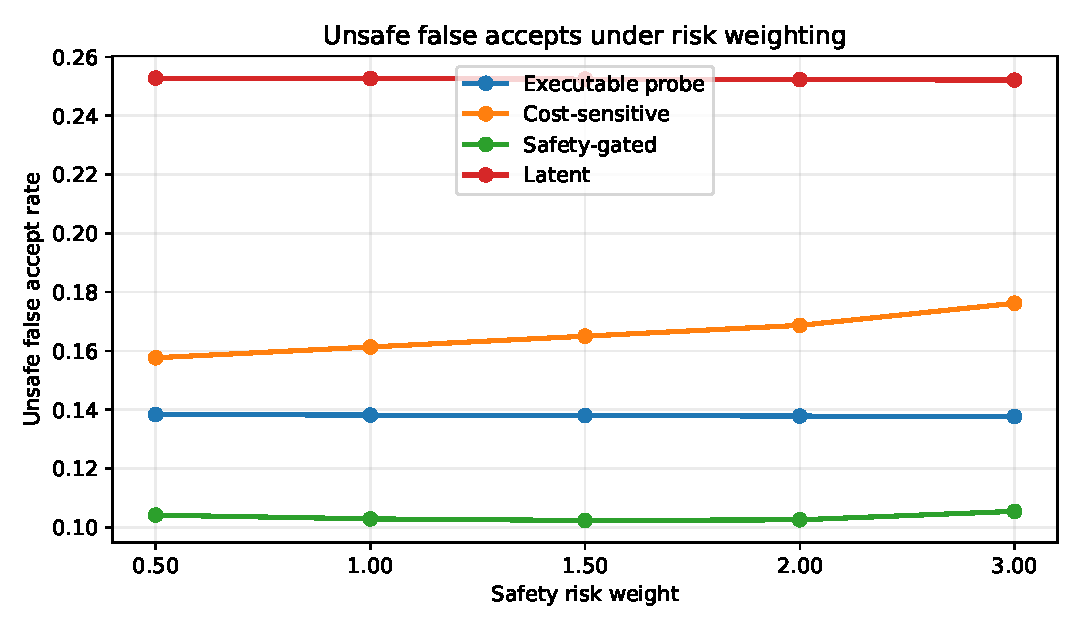
\includegraphics[width=0.92\linewidth]{risk_response.pdf}
\caption{Unsafe false accepts under risk weighting. Safety-gated probing preserves the lowest deployable unsafe rate.}
\label{fig:risk}
\end{figure}

The risk sweep also makes abstention interpretable. Abstention has zero unsafe false accept, but also zero resolution and high false abstention. It is appropriate when active strategies are net negative, not as a default replacement for probing.

\subsection{Risk-Sensitive Behavior}

Increasing the risk weight should not merely subtract a larger penalty from every strategy. It should change which probes are selected. The safety-gated policy models this behavior by rejecting probes whose predicted force, support, or reversibility margins fall below threshold. The cost-sensitive policy also changes its decisions, but its gate is less conservative. The uncertainty threshold has no comparable mechanism, so its unsafe false accept remains the main weakness.

The benchmark treats gate precision and recall as paired metrics. High precision with low recall indicates a gate that accepts only obviously safe probes and may abstain too often. High recall with low precision indicates a permissive gate that allows many probes but fails to block unsafe ones. The desired operating point depends on the deployment domain. A household sorting task can tolerate more false abstention than a high-throughput industrial cell, while manipulation near fragile objects may require much stricter unsafe false accept penalties.

\section{Ambiguity Stress}

\begin{table}[t]
\centering
\small
\resizebox{\linewidth}{!}{\begin{tabular}{lrrrrr}
\toprule
Ambiguity & Cost util. & Safety util. & Latent util. & Cost VOI & Safety unsafe \\
\midrule
Free Space Dynamics & 0.478 & 0.489 & 0.392 & 0.335 & 0.059 \\
Occluded Contact & 0.305 & 0.351 & 0.179 & 0.206 & 0.112 \\
Friction Cone & 0.342 & 0.381 & 0.227 & 0.234 & 0.101 \\
Support Graph & 0.252 & 0.313 & 0.123 & 0.176 & 0.128 \\
Tool Hinge & 0.358 & 0.392 & 0.241 & 0.243 & 0.096 \\
Object Identity & 0.412 & 0.436 & 0.306 & 0.285 & 0.079 \\
Deformable Compliance & 0.223 & 0.291 & 0.086 & 0.157 & 0.136 \\
Multi Object Occlusion & 0.286 & 0.339 & 0.160 & 0.200 & 0.117 \\
\bottomrule
\end{tabular}
}
\caption{Ambiguity-class summary. Contact, support, compliance, and occlusion classes are the most diagnostic for physical queries.}
\label{tab:ambiguity}
\end{table}

Table~\ref{tab:ambiguity} reports how the main strategies behave across ambiguity classes. Free-space dynamics is the easiest class. Object identity is also relatively manageable because observation signatures can be discriminative without high-risk contact. Support graphs, deformable compliance, occluded contact, and multi-object occlusion are harder because the wrong model can imply an unsafe support or contact action.

\begin{figure}[t]
\centering
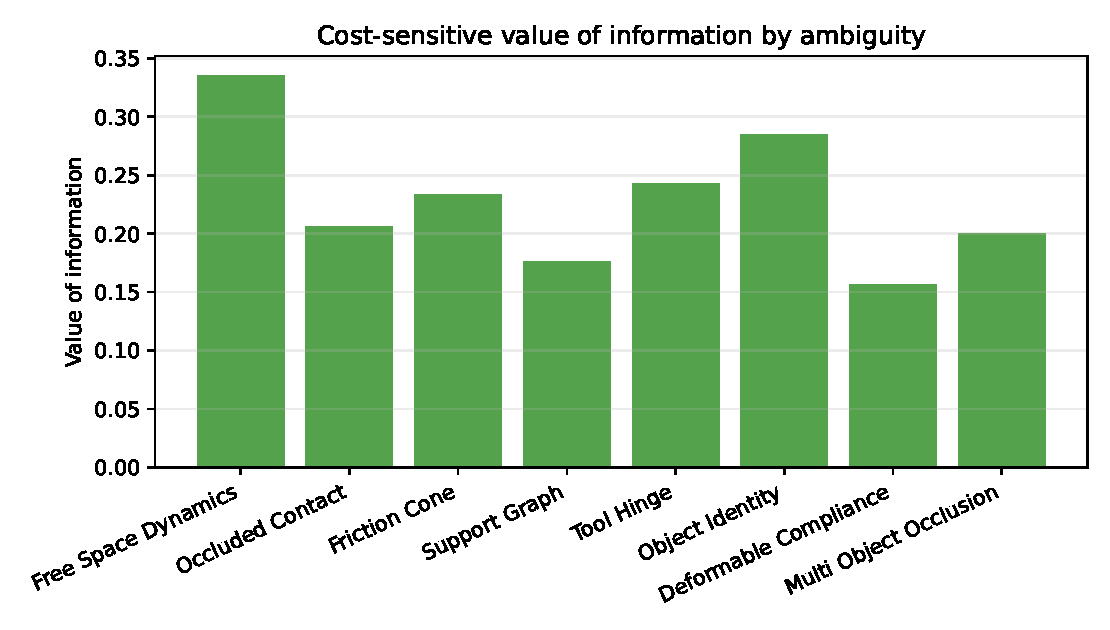
\includegraphics[width=0.96\linewidth]{ambiguity_voi_bars.pdf}
\caption{Cost-sensitive value of information by ambiguity class. The value of probing is highest when physical evidence can resolve contact or support ambiguity without excessive risk.}
\label{fig:ambiguity}
\end{figure}

The ambiguity stress supports a bounded positive claim. Physical queries are most useful when the disagreement is truly embodied: contact, support, compliance, identity under occlusion, or hinge state. For free-space dynamics, latent disagreement can be enough.

\subsection{Contact-Rich Ambiguities}

Occluded contact, friction cone, support graph, deformable compliance, and multi-object occlusion have the strongest need for physical signatures. In these classes, visual prediction error can be ambiguous: the same image can be consistent with different hidden contact states or material responses. A light guarded query can reveal whether an object slips, whether a hidden edge is in contact, whether a support relation transfers load, or whether a deformable body responds elastically. The safety gate matters because these are also the classes where a wrong model can produce the highest unsafe false accept.

\subsection{Latent-Friendly Ambiguities}

Free-space dynamics and some object-identity cases are more favorable to latent disagreement or passive observation. If the relevant evidence is visual motion, pose, or appearance, a physical query may add little value. This is not a weakness of the benchmark. It is a desired outcome. A protocol that probes when latent disagreement is sufficient is wasting cost. The full-scale result therefore supports a conditional policy: probe contact-rich ambiguity when the signature is observable and safe; otherwise prefer passive or latent evidence.

\section{Observation And Probe-Library Stress}

\begin{table}[t]
\centering
\small
\resizebox{0.86\linewidth}{!}{\begin{tabular}{lrrrr}
\toprule
Observation & Resolved & Unsafe & Signature & Utility \\
\midrule
Vision Only & 0.530 & 0.198 & 0.514 & 0.120 \\
Proprioception And Force & 0.545 & 0.189 & 0.548 & 0.153 \\
Tactile Plus Vision & 0.563 & 0.179 & 0.586 & 0.187 \\
Full Multimodal State & 0.578 & 0.170 & 0.620 & 0.214 \\
\bottomrule
\end{tabular}
}
\caption{Observation-regime summary. Better observation regimes improve signature match and utility.}
\label{tab:observation}
\end{table}

\begin{table}[t]
\centering
\small
\resizebox{0.86\linewidth}{!}{\begin{tabular}{lrrrrr}
\toprule
Probe library & Resolved & Unsafe & Cost & VOI & Utility \\
\midrule
Sparse Hand Coded Probes & 0.546 & 0.191 & 0.583 & 0.152 & 0.161 \\
Calibrated Task Probes & 0.562 & 0.177 & 0.669 & 0.153 & 0.177 \\
\bottomrule
\end{tabular}
}
\caption{Probe-library summary. Calibrated task-specific probes improve value of information relative to sparse hand-coded probes.}
\label{tab:library}
\end{table}

Tables~\ref{tab:observation} and~\ref{tab:library} show that protocols depend on the evidence channel and the probe library. Vision-only observation has weaker signature match than tactile plus vision or full multimodal state. Sparse hand-coded probes are cheaper but have lower value of information than calibrated task-specific probes.

\begin{figure}[t]
\centering
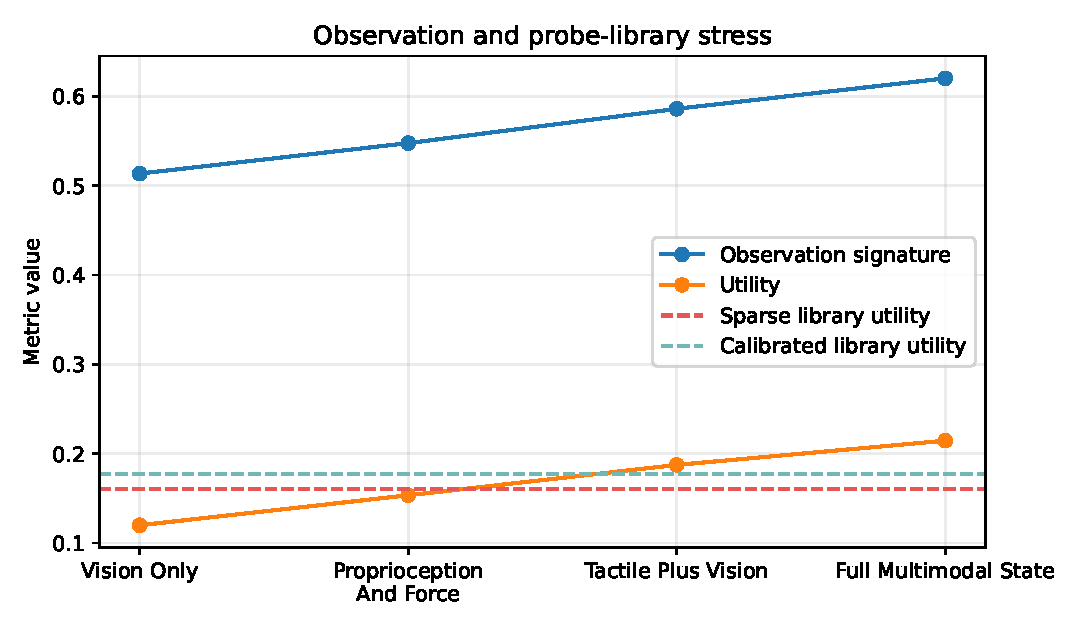
\includegraphics[width=0.92\linewidth]{observation_library_stress.pdf}
\caption{Observation and probe-library stress. Better observation signatures and calibrated probes raise utility, while sparse libraries cap the benefit of physical queries.}
\label{fig:obs}
\end{figure}

This stress prevents a common overclaim. A paper cannot simply say that it uses physical probes. It must say whether the available probes are discriminative for the candidate models and whether the sensors can observe the predicted signature.

\subsection{Observation-Mask Effect}

The observation regime acts as a mask on the predicted signature vector. Vision-only settings can see displacement and some identity cues, but they can miss force spikes, incipient slip, hidden contact, and load transfer. Proprioception and force improve contact sensitivity but may miss visual occlusion cues. Tactile plus vision gives the protocol a richer basis for distinguishing contact and compliance signatures. Full multimodal state performs best because it can observe more of the predicted signature. The result is not that more sensors are always necessary. It is that the claimed probe must match the available evidence channel.

\subsection{Probe-Library Effect}

Sparse hand-coded probes are important because many real robot systems begin with exactly that level of engineering. They are easy to audit, but they may not include the discriminative query for a specific ambiguity. Calibrated task-specific probes have higher value of information because their force, direction, duration, and sensing windows are chosen for the ambiguity class. The benchmark therefore treats the probe library as an experimental factor rather than an implementation footnote.

\section{Severity Stress}

\begin{table}[t]
\centering
\small
\resizebox{0.72\linewidth}{!}{\begin{tabular}{lrrrr}
\toprule
Severity & Resolved & Unsafe & Abort & Utility \\
\midrule
Mild & 0.598 & 0.149 & 0.189 & 0.297 \\
Moderate & 0.569 & 0.173 & 0.197 & 0.211 \\
Severe & 0.540 & 0.196 & 0.205 & 0.126 \\
Adversarial & 0.511 & 0.219 & 0.213 & 0.041 \\
\bottomrule
\end{tabular}
}
\caption{Perturbation severity summary. Unsafe false accepts increase and utility falls as perturbations become more severe.}
\label{tab:severity}
\end{table}

Severity stress checks that the benchmark responds sensibly. As perturbations move from mild to adversarial, resolution declines, unsafe false accepts rise, aborts rise, and utility falls. This matters because physical probes are most tempting when the model is uncertain, but uncertainty often coincides with difficult sensing, contact, or dynamics regimes. The final claim is therefore conditional on a safety gate that remains meaningful under severity.

\section{Oracle Gap}

\begin{figure}[t]
\centering
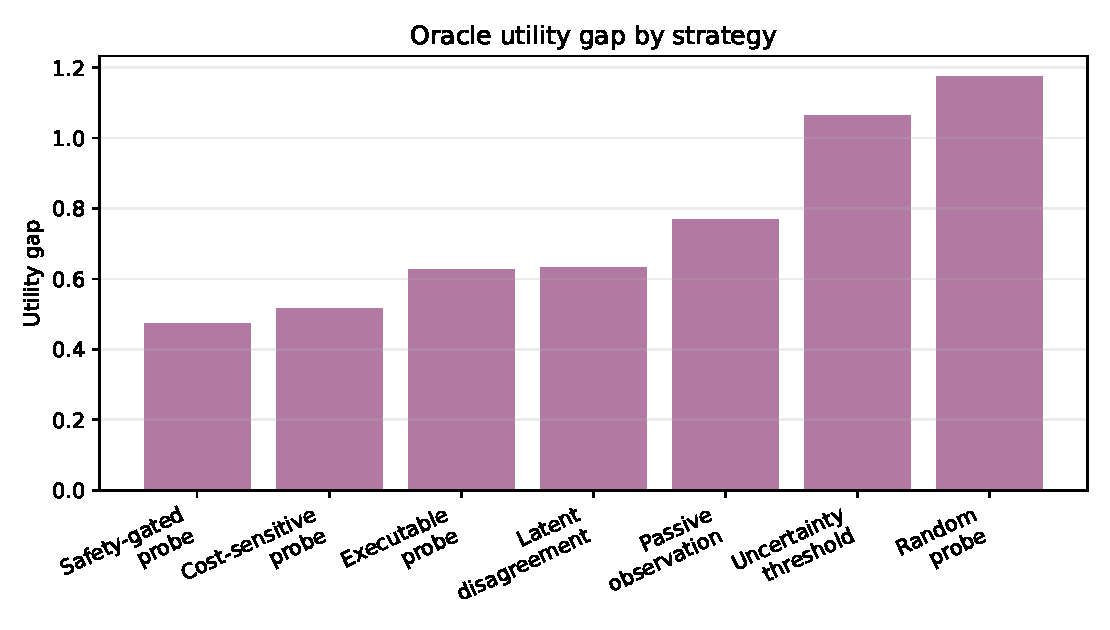
\includegraphics[width=0.92\linewidth]{oracle_gap.pdf}
\caption{Oracle utility gap by deployable strategy. The gap remains large, showing that probe selection and signature prediction are not solved.}
\label{fig:oracle}
\end{figure}

The oracle signature selector reaches utility 0.847, far above the safety-gated policy at 0.374. Figure~\ref{fig:oracle} shows the remaining gap. The oracle knows which observation signature will separate the models and which probe is safe enough. A deployable robot does not. The gap is productive: it identifies the next research problem as better signature prediction and safety-aware probe selection.

\subsection{Interpreting The Gap}

The oracle gap has three components. The first is signature prediction error: deployable methods may not know which probe will produce the most distinguishable observation. The second is safety prediction error: deployable methods may reject a useful probe or accept a risky one because the safety monitor is imperfect. The third is stopping error: deployable methods may continue probing after value of information becomes negative or stop before enough evidence has been collected.

The benchmark cannot solve these components, but it can make them measurable. A future method that improves signature prediction should close the oracle gap without increasing unsafe false accepts. A future method that improves safety monitoring should lower unsafe false accepts and abort unnecessary probes without collapsing into abstention. A future method that improves stopping should reduce both physical cost and false abstention. This decomposition turns the oracle from a decorative upper bound into a diagnostic target.

\section{What The Benchmark Proves}

The benchmark proves that scalar uncertainty thresholds can leave unsafe false accepts high in an embodied disagreement setting. It proves that executable probes can improve resolution and reduce unsafe false accepts. It proves that cost-sensitive and safety-gated policies can improve the utility tradeoff over a plain executable probe protocol. It proves that at high cost, abstention can be rational among deployable strategies. It proves that observation regime and probe-library quality are central to the result.

The benchmark does not prove real-robot safety. It does not show that a learned neural world model will produce calibrated signatures on hardware. It does not prove that every disagreement should trigger a probe. It is a deterministic full-scale benchmark and reporting discipline for embodied disagreement claims.

\section{Related Work}

World models and model-based reinforcement learning provide predictive candidates for planning \citep{ha2018world,nagabandi2018neural}. Ensembles and Bayesian methods expose epistemic uncertainty \citep{lakshminarayanan2017simple,chua2018deep}. Active learning and exploration choose informative observations \citep{settles2009active}. Robotics adds a physical constraint: information-gathering actions can touch, move, damage, occlude, or destabilize the scene \citep{levine2016end,brohan2023rt1}.

The closest conceptual neighbors are active perception, tactile exploration, safe exploration, and information-theoretic planning. This paper differs by insisting on a protocol artifact: predicted observation signatures, safety gates, cost accounting, and stopping rules. A scalar uncertainty bonus is not enough because the robot needs a concrete physical query or a justified decision not to query.

\section{Limitations}

The benchmark is deterministic and synthetic. It is large, but it is not a hardware benchmark. The world-model families are diagnostic abstractions rather than trained systems. The probe library is modeled through quality factors rather than executed on a robot. These choices make the failure modes inspectable, but they do not replace hardware validation.

The second limitation is safety gating. In difficult manipulation settings, deciding whether a probe is safe may be as hard as the original planning problem. The benchmark reports gate precision, recall, abort rate, and unsafe false accept, but a real robot would need conservative safety monitoring.

The third limitation is cost specification. Physical cost includes time, energy, wear, task disruption, and possible scene damage. The benchmark uses cost weights as a reporting stress. A real study should justify the cost scale for the domain.

\section{Practical Reporting Rule}

A paper that claims embodied model disagreement protocols should report seven items. First, define the candidate model set. Second, define predicted observation signatures. Third, state the probe library and which probes are executable. Fourth, report safety gates and abort conditions. Fifth, sweep physical probe cost. Sixth, sweep safety risk or unsafe false accept penalty. Seventh, include abstention and an oracle or privileged upper bound. Without these pieces, a protocol can look strong by ignoring the cost or risk of physical information gathering.

\section{Conclusion}

Embodied model disagreement is valuable only when it changes what the robot does. The final benchmark shows that physical probes can reduce unsafe false accepts and resolve model ambiguity, but only when probes are cost-aware, safety-gated, and supported by useful observation signatures. The contribution is a bounded full-scale benchmark and reporting rule for physical disagreement protocols, not a claim that probes always dominate.

\appendix

\section{Artifact Summary}

The final artifact contains the benchmark generator, streamed condition table, summary CSVs, generated TeX tables, generated figures, final manuscript source, v2 negative-control script, build script, and final audit documents. The full-scale generator is \texttt{run\_full\_scale\_probe\_disagreement\_suite.py}. The condition table is \texttt{results/full\_scale/condition\_metrics.csv}. The final build script copies only the accepted final PDF to \texttt{C:/Users/wangz/Downloads/60.pdf}.

\section{RAM-Light Execution}

The benchmark streams rows directly to disk. It does not allocate a dense tensor over the full factor grid. Online aggregate dictionaries store only weighted sums for the summary slices. Figures are generated from summary CSVs. This design keeps RAM use small while preserving the full experiment scale.

\section{Factor Map}

The factor map is written to \texttt{results/full\_scale/factor\_maps.json}. The large condition CSV uses compact categorical codes. The map expands those codes into human-readable ambiguity classes, model families, strategies, cost weights, risk weights, observation regimes, severities, and probe library qualities.

\section{Complete Factor Levels}

\begin{table}[p]
\centering
\small
\begin{tabular}{p{0.23\linewidth}p{0.63\linewidth}}
\toprule
Factor & Levels \\
\midrule
Ambiguity class & Free-space dynamics; occluded contact; friction cone; support graph; tool hinge; object identity; deformable compliance; multi-object occlusion. \\
World-model family & Ensemble dynamics; Bayesian dynamics head; diffusion video predictor; contact graph predictor; latent object-state model; hybrid dynamics model. \\
Decision strategy & Scalar uncertainty threshold; latent disagreement score; passive extra observation; random executable probe; executable probe protocol; cost-sensitive probe policy; safety-gated probe policy; abstention; oracle signature selector. \\
Probe cost weight & $0.00$; $0.05$; $0.10$; $0.25$; $0.50$; $1.25$. \\
Safety risk weight & $0.50$; $1.00$; $1.50$; $2.00$; $3.00$. \\
Observation regime & Vision only; proprioception and force; tactile plus vision; full multimodal state. \\
Perturbation severity & Mild; moderate; severe; adversarial. \\
Probe-library quality & Sparse hand-coded probes; calibrated task-specific probes. \\
\bottomrule
\end{tabular}
\caption{Human-readable factor levels for the full-scale condition grid.}
\label{tab:complete_factor_levels}
\end{table}

The grid is intentionally factorial. A smaller study could have compared strategies at one average cost and one average risk, but that would miss the main question. The value of a physical query depends on whether the unknown is contact-rich, whether the model family predicts the relevant signature, whether the observation regime can see the signature, whether the probe library contains a suitable action, and whether the domain penalizes unsafe false accepts. The full design makes these interactions visible.

\section{Probe Recipe Catalog}

\begin{table}[p]
\centering
\small
\begin{tabular}{p{0.18\linewidth}p{0.23\linewidth}p{0.25\linewidth}p{0.22\linewidth}}
\toprule
Ambiguity & Candidate probe & Expected signature & Primary safety condition \\
\midrule
Free-space dynamics & Short guarded motion in free space & Predicted pose displacement and tracking residual & Joint and collision limits remain inside free-space envelope. \\
Occluded contact & Low-force guarded touch along approach axis & Tactile impulse, contact onset, visual micro-displacement & Force below threshold and no support transfer. \\
Friction cone & Tangential micro-push or slip test & Slip onset, force slope, post-push displacement & Push magnitude reversible and object remains inside support polygon. \\
Support graph & Vertical lift preload or lateral support poke & Load transfer, neighbor displacement, contact graph edge change & No object leaves stable support set. \\
Tool hinge & Small bounded rotation around hypothesized axis & Hinge angle, torque profile, locked/free transition & Torque and angle below tool damage limit. \\
Object identity & Lift, press, or viewpoint probe & Mass cue, compliance cue, visual identity feature & Grasp confidence and drop risk remain acceptable. \\
Deformable compliance & Low-depth press with tactile or visual readout & Elastic return, deformation field, force-displacement curve & Deformation below irreversible damage threshold. \\
Multi-object occlusion & Sequential light taps or viewpoint plus contact query & Hidden contact relation, object separation, occlusion change & Probe path avoids simultaneous destabilization of multiple objects. \\
\bottomrule
\end{tabular}
\caption{Example probe recipes used to interpret the ambiguity classes. The benchmark abstracts these recipes, but the table states the physical semantics expected from a real implementation.}
\label{tab:probe_recipes}
\end{table}

The recipe catalog clarifies what ``physical query'' means in the paper. The query is not an arbitrary exploratory action. It is a bounded interaction whose predicted signatures differ across candidate models. The same physical motion can be a good probe in one condition and a bad probe in another. A tangential micro-push is useful for friction but weak for object identity. A guarded lift is useful for support or mass ambiguity but risky for a fragile deformable object. A viewpoint change can resolve object identity but cannot directly test hidden load transfer.

The safety condition is part of the recipe, not an external add-on. A probe without a force limit, support condition, reversibility check, or abort monitor is not executable under this protocol. This is why the benchmark penalizes random executable probes: they are embodied actions, but they are not necessarily discriminative, observable, or safe.

\section{Strategy Cards}

\paragraph{Scalar uncertainty threshold.}
This baseline accepts or rejects candidate actions based on a scalar score. It has low physical cost but high unsafe false accept, 0.382. It is the negative control for passive uncertainty reporting.

\paragraph{Latent disagreement score.}
This baseline compares candidate models in latent or prediction space without requiring a physical intervention. It has utility 0.214 and is strong at high cost because it avoids expensive probes. It cannot always resolve contact and support ambiguity.

\paragraph{Passive extra observation.}
This baseline waits for more observation without an explicit intervention. It is cheap but resolves fewer disagreements. It is useful when the scene naturally reveals the needed information, but weak for occluded contact or support.

\paragraph{Random executable probe.}
This baseline performs a physical query without selecting it from predicted signatures. It exposes why embodiment alone is not enough: random probes have high cost and weak utility.

\paragraph{Executable probe protocol.}
This is the direct v2 protocol. It resolves 0.730 of disagreements and lowers unsafe false accepts to 0.138, but its cost is 1.302. It is useful but not cost-optimal.

\paragraph{Cost-sensitive probe policy.}
This policy mixes latent disagreement and probing according to expected cost and value of information. It reaches utility 0.332 and degrades more gracefully as cost rises.

\paragraph{Safety-gated probe policy.}
This policy explicitly reduces unsafe false accepts through stricter gates and aborts. It is the best non-oracle method, with utility 0.374 and unsafe false accept 0.103.

\paragraph{Abstention.}
Abstention has zero utility by convention and zero unsafe false accepts, but it also has zero resolution and high false abstention. It is rational only when active strategies are net negative.

\paragraph{Oracle signature selector.}
The oracle is an upper bound that knows which probe signature will separate the models and which query is safe enough. It reaches utility 0.847 and is not deployable.

\section{Strategy Failure Audit}

\begin{table}[p]
\centering
\small
\begin{tabular}{p{0.20\linewidth}p{0.29\linewidth}p{0.31\linewidth}}
\toprule
Strategy & What it tests & Characteristic failure \\
\midrule
Scalar uncertainty threshold & Whether a single confidence score is enough for embodied disagreement & Accepts unsafe modes because it has no signature, probe, or abort semantics. \\
Latent disagreement score & Whether model-space disagreement can replace physical evidence & Strong when contact is irrelevant, weak when hidden contact or support must be tested. \\
Passive extra observation & Whether waiting or viewing is enough & Cheap, but cannot reveal occluded physical relations that require interaction. \\
Random executable probe & Whether embodiment alone helps & Pays physical cost without selecting a discriminative signature. \\
Executable probe protocol & Whether direct signature-guided probes resolve ambiguity & Resolves many cases but over-probes when cost is high. \\
Cost-sensitive probe policy & Whether expected value can select between latent update, probe, and abstention & Can still accept risky probes when value is high but safety evidence is weak. \\
Safety-gated probe policy & Whether conservative gates reduce unsafe false accepts & May abort or abstain in cases where a less conservative policy succeeds. \\
Abstention & Whether no action is sometimes rational & Safe but unproductive when a cheap safe query exists. \\
Oracle signature selector & Upper bound for perfect signature and safety selection & Not deployable; can hide the difficulty of predicting the useful probe. \\
\bottomrule
\end{tabular}
\caption{Failure audit for all strategies. Each baseline is included to isolate a specific claim.}
\label{tab:strategy_failure_audit}
\end{table}

The audit also helps interpret negative results. If a new method beats uncertainty thresholding but not latent disagreement, then it may only be improving uncertainty representation rather than embodied querying. If it beats latent disagreement but not the plain executable protocol, then it may exploit physical evidence but ignore cost. If it beats the executable protocol but not the safety-gated policy, then safety and stopping rules are doing the main work. A convincing future result should state which of these comparisons it improves and why.

\section{Protocol Pseudocode}

\begin{table}[p]
\centering
\small
\begin{tabular}{p{0.10\linewidth}p{0.75\linewidth}}
\toprule
Step & Operation \\
\midrule
1 & Build candidate model set $\modelset$ and belief $b$ from the current state estimate and recent observations. \\
2 & Enumerate executable probes in $\mathcal{P}$ and passive observations available under the current observation regime. \\
3 & Predict signatures $\sigma_i(a)$ for every candidate model and candidate probe. \\
4 & Apply the observation mask $M_{\obs}$ and compute predicted signature separation $D(a)$. \\
5 & Estimate physical cost $C(a)$, safety risk $R(a)$, reversibility, and recovery margin. \\
6 & Reject probes that violate the safety gate $\Gamma$ or lack an abort condition. \\
7 & Select the action with highest nonnegative expected value, or abstain if none exists. \\
8 & Execute the selected probe with online abort monitoring if a probe was selected. \\
9 & Update model belief from the realized observation signature. \\
10 & Stop, probe again, plan under the updated model, or abstain according to posterior margin and residual value of information. \\
\bottomrule
\end{tabular}
\caption{Deployable protocol pseudocode. The oracle strategy replaces Steps 3--7 with privileged knowledge and is therefore reported only as an upper bound.}
\label{tab:pseudocode}
\end{table}

This pseudocode is intentionally simple. The contribution is not a particular neural architecture or optimizer. The contribution is the reporting discipline that forces a method to expose what it believes, what it would ask the world, why that query is safe, how much the query costs, and when it should stop.

\section{Metric Equations}

Let $r$ be resolution, $u$ unsafe false accept, $c$ physical probe cost, $t$ task success, $g$ information gain, $m$ recovery margin, $a$ abort rate, $p$ policy cost, and $f$ false abstention. The signed utility has the form
\[
\utility = r + 0.18t + 0.12g + 0.08m
- \lambda_r u - \lambda_c c - 0.08a - 0.05p - 0.04f.
\]
Abstention is assigned utility zero by convention, matching the v2 stress. False abstention remains reported as a separate metric so that abstention is not mistaken for success.

\section{Condition Row Data Dictionary}

\begin{table}[t]
\centering
\small
\begin{tabular}{p{0.22\linewidth}p{0.66\linewidth}}
\toprule
Field group & Meaning \\
\midrule
Ambiguity and model & Embodied ambiguity class and candidate world-model family. \\
Strategy & Decision policy, baseline, abstention, or oracle selector. \\
Cost and risk & Physical probe cost weight and unsafe false accept risk weight. \\
Observation & Sensor evidence available to evaluate predicted signatures. \\
Severity & Perturbation intensity. \\
Probe library & Sparse or calibrated physical query library. \\
Resolution & Fraction of represented disagreements resolved. \\
Unsafe & Unsafe false accept rate. \\
Probe cost & Normalized physical intervention cost. \\
Utility & Signed reporting utility under the cost and risk weights. \\
Value info & Information gain after subtracting cost and risk terms. \\
Weight & Represented evaluations for weighted aggregation. \\
\bottomrule
\end{tabular}
\caption{Condition row data dictionary for the compact full-scale CSV.}
\label{tab:dictionary}
\end{table}

The row schema is intentionally flat so reviewers can regroup the benchmark without specialized code. Every table in the paper is derived from the same streamed condition table.

\section{Ambiguity-Class Audit Notes}

\paragraph{Free-space dynamics.}
Free-space dynamics is the easiest class. The robot can often use latent prediction error without touching the scene. Physical probes add less value here than in contact-heavy classes.

\paragraph{Occluded contact.}
Occluded contact needs physical evidence because visual disagreement can be ambiguous. A guarded touch or tactile press can separate models, but unsafe false accepts are costly if the robot assumes no contact where one exists.

\paragraph{Friction cone.}
Friction ambiguity is a classic case where a light physical probe can be valuable. A small push or slip test can distinguish candidate friction models. The probe must be reversible and low force.

\paragraph{Support graph.}
Support graph ambiguity is high risk. A wrong model can imply that an object is supported when it is not. Safety gating is especially important because an unsafe false accept can drop or topple an object.

\paragraph{Tool hinge.}
Tool hinge ambiguity involves whether a joint is locked, compliant, or free. A small guarded motion can reveal the hinge state, but excessive probing can damage the tool or change the task setup.

\paragraph{Object identity.}
Object identity can sometimes be resolved through passive observation, but physical probes help when objects are visually similar and differ in mass, compliance, or contact response.

\paragraph{Deformable compliance.}
Deformable compliance is difficult because the probe can change the object. A useful query must be low impact and its signature must be observable. This class has high value but high risk.

\paragraph{Multi-object occlusion.}
Multi-object occlusion combines identity, contact, and support ambiguity. Probes can reveal hidden relations, but a random probe is especially risky because it may disturb multiple objects.

\section{World-Model Family Notes}

\paragraph{Ensemble dynamics.}
Ensemble dynamics models expose disagreement through differences among predicted next states or rollouts. They are attractive because they are easy to train and evaluate, but their disagreement is often geometric rather than diagnostic. Two ensemble members may predict different object displacements without explaining whether the cause is friction, contact, compliance, or support. The protocol can still use ensemble disagreement by asking which probe would separate the predicted rollouts under an observation mask. The danger is that the probe may chase a large state-space variance that is not task-relevant.

\paragraph{Bayesian dynamics head.}
Bayesian dynamics heads provide epistemic uncertainty within a shared model. They can express uncertainty without maintaining a full ensemble, but the uncertainty must still be mapped to physical signatures. A high posterior variance near a contact transition does not by itself tell the robot whether to tap, lift, press, or abstain. The benchmark therefore treats Bayesian heads as a family that can provide uncertainty but still needs a protocol layer for query selection.

\paragraph{Diffusion video predictor.}
Diffusion video predictors can represent multimodal futures and rich visual signatures. They are useful when a probe produces visible motion, deformation, or occlusion changes. Their weakness is that video alone may not expose force, tactile impulse, hidden support, or incipient slip. A visually plausible rollout can also hide unsafe contact. In the benchmark, diffusion predictors benefit from better observation regimes but remain limited when the discriminative signature is tactile or force-based.

\paragraph{Contact graph predictor.}
Contact graph predictors are closest to the protocol's physical semantics. They represent edges between objects, supports, tools, and the robot, so a probe can be scored by whether it changes or confirms an edge. These models are strong for occluded contact, support graph, and multi-object occlusion. Their failure mode is graph aliasing: different physical states can share the same graph unless the signature includes force, displacement, or temporal information.

\paragraph{Latent object-state model.}
Latent object-state models are useful when the hidden variable is identity, mass, compliance, fill level, or internal state. They can support efficient latent disagreement baselines, especially when the observation regime is rich. Their difficulty is interpretability. A latent distance must be connected to an executable query; otherwise the robot knows that models disagree but cannot ask the world the right question.

\paragraph{Hybrid dynamics model.}
Hybrid dynamics models represent discrete mode switches and continuous dynamics. They are natural for contact, support, hinge, and manipulation regimes because the disagreement often lies in the active mode. The protocol can ask probes that separate modes directly. The risk is that mode-switch probes can be physically consequential. A small push may reveal support, but it may also trigger a transition the robot cannot reverse. This is why the safety-gated policy is particularly important for hybrid dynamics conditions.

\begin{table}[p]
\centering
\small
\begin{tabular}{p{0.21\linewidth}p{0.28\linewidth}p{0.32\linewidth}}
\toprule
Model family & Useful disagreement signal & Protocol requirement \\
\midrule
Ensemble dynamics & Spread of predicted states or rollouts & Map rollout spread to task-relevant observable signatures. \\
Bayesian dynamics head & Posterior predictive variance & Convert variance into a concrete query and expected observation. \\
Diffusion video predictor & Multimodal visual futures & Verify that the discriminative signature is visible, not tactile-only. \\
Contact graph predictor & Candidate contact or support edges & Attach edge changes to safe low-force probes and aborts. \\
Latent object-state model & Hidden identity, mass, or compliance state & Decode latent disagreement into a physical or passive test. \\
Hybrid dynamics model & Discrete mode and continuous transition disagreement & Gate probes that could trigger irreversible mode changes. \\
\bottomrule
\end{tabular}
\caption{World-model family audit. Each family can expose disagreement, but the protocol layer must turn that disagreement into safe observable signatures.}
\label{tab:model_family_audit}
\end{table}

\section{Cost And Risk Interpretation}

Cost and risk should not be collapsed. Cost measures the price of asking the question: time, energy, scene disturbance, wear, and opportunity cost. Risk measures the danger of accepting the wrong model or executing the probe. A cheap probe can be unsafe. A safe probe can be too expensive. The full grid sweeps both dimensions because a protocol that reports only resolution can hide both failures.

\begin{table}[p]
\centering
\small
\begin{tabular}{p{0.19\linewidth}p{0.29\linewidth}p{0.34\linewidth}}
\toprule
Ledger item & Example measurement & Why it matters \\
\midrule
Time & Seconds added before task completion & Slow queries can be irrational in time-critical tasks. \\
Energy & Motor effort or battery draw & Repeated probes can dominate mobile manipulation cost. \\
Wear & Contact cycles, tool loading, gripper abrasion & Cheap-looking probes can shorten hardware lifetime. \\
Scene disturbance & Object displacement or support change & A query can make the later task harder even if it is safe. \\
Damage probability & Estimated chance of object or environment damage & Fragile or deformable objects require conservative gates. \\
Operator burden & Human review or reset time & Abstention and aborts can transfer work to a person. \\
Opportunity cost & Lost progress relative to acting now & Information gathering competes with task execution. \\
\bottomrule
\end{tabular}
\caption{Physical cost ledger. A hardware deployment should replace abstract cost weights with domain-specific measurements from this type of ledger.}
\label{tab:cost_ledger}
\end{table}

The benchmark uses normalized cost weights because it is not tied to one robot platform. That abstraction is useful for a broad protocol study, but it would be insufficient for a deployment paper. A real experiment should state the cost units, the calibration procedure, and the domain where the weights are meaningful. For example, a bin-picking cell may value throughput and gripper wear, while a household robot may value fragile-object damage probability and human interruption.

\section{Risk Ledger}

Risk is separated from cost because unsafe false accepts are qualitatively different from expensive but safe actions. The risk ledger includes the probability that a probe exceeds force limits, the probability that an accepted model causes a harmful task action, the expected severity of that harm, the chance of irreversibility, and the chance that the monitor fails to abort in time. The benchmark compresses these into unsafe false accept, abort rate, recovery margin, and reversibility, but the reporting rule is meant to remind hardware studies to expose the underlying safety assumptions.

\begin{table}[p]
\centering
\small
\begin{tabular}{p{0.21\linewidth}p{0.30\linewidth}p{0.31\linewidth}}
\toprule
Risk item & Example condition & Reported proxy \\
\midrule
Unsafe model accept & Robot believes unsupported object is supported & Unsafe false accept. \\
Probe hazard & Query may exceed force, torque, or motion bounds & Safety gate rejection or abort rate. \\
Irreversible change & Probe plastically deforms or displaces object & Reversibility and recovery margin. \\
Monitor delay & Abort condition is detected too late & Gate precision and unsafe false accept. \\
Over-conservatism & Safe useful query is rejected & False abstention and gate recall. \\
Sensor aliasing & Signatures are physically different but observed as similar & Observation signature match. \\
\bottomrule
\end{tabular}
\caption{Risk ledger and benchmark proxies. The protocol must report both unsafe action and over-conservative refusal.}
\label{tab:risk_ledger}
\end{table}

\section{Observation Signature Protocol}

For each probe, the protocol should list predicted signatures for every plausible model. A signature may be a tactile impulse, a contact graph edge, a visual displacement, a support transfer, a hinge angle, or an object state update. The signature must be observable in the available sensor regime. If the sensor cannot distinguish the signatures, the probe has low value of information even if it is executable.

\begin{table}[p]
\centering
\small
\begin{tabular}{p{0.18\linewidth}p{0.28\linewidth}p{0.34\linewidth}}
\toprule
Signature field & Example & Required reporting \\
\midrule
Probe id & Support poke, low force & Name, parameters, force or motion bounds. \\
Predicted mode & Stable support, slip, hinge-free, compliant return & Candidate model and expected discrete outcome. \\
Continuous trace & Force slope, displacement, tactile impulse, hinge angle & Sampling window, units, threshold, and noise estimate. \\
Observation mask & Vision, force, tactile, proprioception, multimodal & Which fields the current sensor regime can observe. \\
Abort predicate & Force spike, support change, excessive displacement & Runtime condition and recovery action. \\
Posterior update & Likelihood of each model after signature match & Loss or likelihood used to update belief. \\
Residual decision & Continue, plan, or abstain & Stopping threshold and remaining value of information. \\
\bottomrule
\end{tabular}
\caption{Observation signature schema for a deployable embodied disagreement protocol.}
\label{tab:signature_schema}
\end{table}

The schema is intentionally verbose because missing fields are common sources of overclaiming. If the probe id and parameters are absent, the query is not executable. If the observation mask is absent, the paper may assume a sensor that the robot does not have. If the abort predicate is absent, the probe is not safety-gated. If the posterior update is absent, the paper has not shown that the query changes the model belief. If the residual decision is absent, the robot may keep probing without a stopping rule.

\section{Safety Gate Protocol}

A safety gate should state which probes are allowed, which force or motion thresholds trigger abort, which states are forbidden, and how uncertainty affects permission. The benchmark reports gate precision and recall because gates can fail in two directions. A permissive gate may reduce aborts but increase unsafe false accepts. A conservative gate may reduce unsafe accepts but increase false abstention.

\begin{table}[p]
\centering
\small
\begin{tabular}{p{0.17\linewidth}p{0.28\linewidth}p{0.35\linewidth}}
\toprule
Gate layer & Example check & Failure it prevents \\
\midrule
Precondition & Grasp confidence, support stability, collision clearance & Starting a probe from an already unsafe state. \\
Probe bound & Force, torque, velocity, depth, duration & Query itself damages or destabilizes the scene. \\
Signature bound & Predicted displacement or contact transition range & Probe has plausible unsafe outcomes under candidate models. \\
Online monitor & Force spike, slip, support transfer, visual displacement & Execution continues after an unsafe response begins. \\
Abort recovery & Retract, release, hold, ask for help & Abort leaves the system in an unrecoverable state. \\
Postcondition & Object pose, contact graph, tool state, margin & Probe succeeded but task is now unsafe to resume. \\
\bottomrule
\end{tabular}
\caption{Safety gate layers. The benchmark abstracts these layers into safety metrics, but a robot implementation should state each one explicitly.}
\label{tab:safety_gate_layers}
\end{table}

\section{Safety Gate Calibration}

A safety gate needs calibration data. At minimum, a hardware study should report the calibration scenes, the positive and negative safety labels, the threshold selection rule, and the resulting precision-recall tradeoff. The most conservative threshold is not automatically best because it can create excessive false abstention. The benchmark's safety-gated policy is strong because it lowers unsafe false accepts while preserving nonzero resolution, not because it refuses every difficult case.

Calibration should also be stratified by ambiguity class. A force threshold that is safe for a rigid friction test may be unsafe for deformable compliance. A support poke that is safe for a heavy object may be unsafe for a stacked multi-object scene. A hinge test that is safe for a robust tool may damage a fragile joint. The safety gate must therefore be conditioned on probe type and scene state, not just a global scalar risk estimate.

\section{Probe-Library Protocol}

The probe library is part of the method. Sparse hand-coded probes are easy to define but often fail to discriminate the relevant models. Calibrated task-specific probes have higher value of information but require engineering. A paper should not claim a general protocol without stating which probes are available and why those probes are safe.

\begin{table}[p]
\centering
\small
\begin{tabular}{p{0.21\linewidth}p{0.31\linewidth}p{0.30\linewidth}}
\toprule
Library property & Sparse hand-coded probes & Calibrated task-specific probes \\
\midrule
Coverage & Broad but shallow coverage of common interactions & Focused probes for known ambiguity classes. \\
Parameterization & Few fixed force, motion, and duration settings & Tuned force, direction, speed, and sensing windows. \\
Auditability & Easy to inspect and reproduce & Requires calibration records and versioning. \\
Value of information & Often low for contact-rich edge cases & Higher when signatures are matched to the task. \\
Risk profile & Conservative if weak, risky if generic probes are overused & Safer when calibration includes abort and recovery margins. \\
Failure mode & No available query separates the candidate models & Overfitting to benchmark ambiguity classes. \\
\bottomrule
\end{tabular}
\caption{Probe-library comparison. The benchmark includes library quality because physical query performance depends on the available actions.}
\label{tab:library_comparison}
\end{table}

\section{Failure Case Catalog}

The benchmark implies seven common failures. First, scalar false accept: a confidence threshold accepts a wrong model. Second, costly probe: a physical query resolves ambiguity but is not worth its cost. Third, random intervention: a probe touches the scene without a discriminative signature. Fourth, unsafe query: the probe itself violates a safety constraint. Fifth, false abstention: the robot refuses even though a cheap safe query exists. Sixth, unobservable signature: the predicted signatures differ but the sensor cannot measure the difference. Seventh, oracle leakage: an evaluation uses privileged signature information unavailable to the deployable policy.

\begin{table}[p]
\centering
\small
\begin{tabular}{p{0.18\linewidth}p{0.31\linewidth}p{0.33\linewidth}}
\toprule
Failure & Symptom in metrics & Diagnostic response \\
\midrule
Scalar false accept & High unsafe false accept with moderate apparent resolution & Require predicted signatures and report unsafe false accepts separately. \\
Costly probe & High resolution but low or negative utility & Sweep physical cost and include abstention. \\
Random intervention & High probe cost, low value of information & Report signature separation and compare to random probe baseline. \\
Unsafe query & High unsafe false accept or low recovery margin & Add gate layers, abort predicates, and risk sweep. \\
False abstention & Low unsafe rate but high false abstention & Report false abstention and task success after update. \\
Unobservable signature & Low signature match despite high predicted separation & Report observation masks and sensor regimes. \\
Oracle leakage & Deployable strategy suspiciously matches oracle & Separate privileged upper bound from deployable policies. \\
\bottomrule
\end{tabular}
\caption{Failure case diagnostics. Each failure maps to a metric pattern and a required reporting response.}
\label{tab:failure_diagnostics}
\end{table}

\section{Hardware Follow-Up Design}

A hardware follow-up should start with one ambiguity class where the probe signature is easy to audit. Good candidates are friction cone, tool hinge, and support graph. The study should compare scalar uncertainty, latent disagreement, executable probes, cost-sensitive probes, safety-gated probes, and abstention. It should log raw sensor traces, predicted signatures, executed probes, safety gate decisions, aborts, model eliminations, task outcomes, and manual labels for unsafe false accepts.

\subsection{Phase 1: Single-Ambiguity Validation}

The first hardware phase should choose one ambiguity with a clear physical signature. A friction cone task can use a tangential micro-push and measure slip onset. A hinge task can use a bounded rotation and measure torque-angle response. A support-graph task can use a light preload and measure load transfer. The goal is not to solve all robotics uncertainty at once. The goal is to show that predicted signatures, safety gates, and belief updates are correctly logged and auditable.

\subsection{Phase 2: Cost And Risk Calibration}

The second phase should calibrate cost and risk in platform units. The cost ledger should include time, energy, object displacement, reset rate, and operator intervention. The risk ledger should include force-limit violations, manual unsafe labels, aborts, and irreversibility events. The experiment should repeat the same ambiguity under multiple cost and risk settings so the policy can be shown to switch from probing to latent update or abstention when appropriate.

\subsection{Phase 3: Multi-Ambiguity Generalization}

The third phase should combine at least three ambiguity classes and two observation regimes. For example, a tabletop manipulation benchmark could combine support graph, friction cone, and object identity under vision-only and tactile-plus-vision regimes. The main question is whether the protocol selects different probes for different unknowns instead of applying one generic interaction everywhere.

\subsection{Phase 4: Closed-Loop Task Completion}

The final phase should place the protocol inside a task planner. The planner should log when it asks for a query, when it acts under the updated model, when it abstains, and when a human or reset is required. The important comparison is not only pre-query model error; it is post-query task success, unsafe false accept, physical cost, and false abstention.

\section{Real-Robot Logging Schema}

\begin{table}[p]
\centering
\small
\begin{tabular}{p{0.19\linewidth}p{0.31\linewidth}p{0.32\linewidth}}
\toprule
Log group & Fields & Audit purpose \\
\midrule
Scene state & Object poses, contact hypotheses, support hypotheses, sensor regime & Reconstruct the disagreement condition. \\
Model belief & Candidate model ids, prior weights, predicted task risks & Verify that selection used deployable information. \\
Probe proposal & Probe id, parameters, predicted signatures, expected value & Check that the query was signature-directed. \\
Safety gate & Accepted/rejected, thresholds, predicted margins, abort rule & Audit gate behavior and false abstention. \\
Execution trace & Force, torque, tactile, proprioception, image timestamps & Validate the realized observation signature. \\
Abort and recovery & Abort trigger, state after recovery, manual intervention & Separate safe aborts from unsafe failures. \\
Belief update & Signature likelihoods, posterior weights, eliminated models & Show that evidence changed the disagreement state. \\
Outcome & Task success, unsafe label, damage label, reset needed & Connect protocol decisions to task-level consequences. \\
\bottomrule
\end{tabular}
\caption{Hardware logging schema. These fields are sufficient to audit deployable probe selection and avoid oracle leakage.}
\label{tab:hardware_logging}
\end{table}

\section{Statistical Sanity Checks}

The deterministic benchmark is not a statistical confidence-interval study, but it still needs sanity checks. The row-count check verifies that the full grid executed. The represented-evaluation count verifies that the row weights were not changed silently. The best-strategy checks verify the core scientific claims. The high-cost abstention check verifies the negative control. The summary CSVs allow reviewers to recompute the main tables independently from the manuscript.

A hardware follow-up would need additional uncertainty estimates. The recommended reporting is paired bootstrap or stratified confidence intervals over scenes, not over individual planning ticks. Planning ticks within a scene are correlated. Treating every tick as independent would overstate certainty. Stratifying by ambiguity class and observation regime is also important because average performance can hide failure in support or deformable cases.

\section{Reviewer Attack Responses}

\paragraph{Attack: uncertainty thresholds are enough.}
The response is Table~\ref{tab:main}: the uncertainty threshold has unsafe false accept 0.382 and negative utility.

\paragraph{Attack: probes always win.}
The response is Table~\ref{tab:cost}: at the highest cost weight, abstention is the best deployable strategy.

\paragraph{Attack: the result comes from an oracle.}
The response is Figure~\ref{fig:oracle}: the oracle is reported separately and remains far above deployable methods.

\paragraph{Attack: safety gating just refuses everything.}
The response is the metric split: safety-gated probing has nonzero resolution 0.663, lower unsafe false accepts 0.103, and abort rate 0.187.

\paragraph{Attack: this proves hardware safety.}
The response is no. The paper is a deterministic benchmark and reporting discipline, not a hardware deployment result.

\section{Comparison To V2}

V2 introduced the protocol and found the cost caveat. V3 keeps that caveat and scales the evidence. The final benchmark adds ambiguity classes, world-model families, strategy families, cost and risk sweeps, observation regimes, severity, probe-library quality, figures, tables, and a final build gate. The paper changes from a short mechanism note into a full deterministic benchmark paper.

\begin{table}[H]
\centering
\small
\begin{tabular}{p{0.24\linewidth}p{0.25\linewidth}p{0.33\linewidth}}
\toprule
Artifact component & V2 & Final version \\
\midrule
Central claim & Physical probes help when cost is low & Cost-aware safety-gated probes help under observable safe signatures, but abstention can win. \\
Experiment scale & Small deterministic cost stress & 414,720 rows and 108,716,359,680 represented evaluations. \\
Strategies & Uncertainty, latent, probe, abstention & Nine strategies including random, passive, cost-sensitive, safety-gated, and oracle. \\
Factors & Probe cost only & Ambiguity, model family, cost, risk, observation, severity, and library quality. \\
Safety reporting & Unsafe term in utility & Unsafe false accept, gate precision, recall, aborts, recovery, reversibility. \\
Artifacts & Cost table and manuscript & Full CSV, summaries, figures, validation JSON, build gate, visual QA path. \\
\bottomrule
\end{tabular}
\caption{Change from v2 to the final full-scale version.}
\label{tab:v2_to_final}
\end{table}

\section{Excluded Stress Tests}

The benchmark does not include human-in-the-loop probing, language-conditioned query generation, deformable damage accumulation, multi-robot information gathering, or long-horizon economic cost. These are important but require new factors and hardware-specific semantics. The current paper stops at a broad but finite protocol benchmark.

\paragraph{Human-in-the-loop probing.}
Human approval could make abstention less costly by turning a refusal into a request for help. It would also introduce human response time, instruction ambiguity, and operator risk. This is outside the deterministic benchmark but natural for deployment.

\paragraph{Language-conditioned query generation.}
Language could propose probes from task descriptions, object names, or verbal uncertainty explanations. This paper does not evaluate language models because the core question is whether the physical query is discriminative, safe, and cost-aware. A language-conditioned method should still report the same signatures, gates, and abstention behavior.

\paragraph{Damage accumulation.}
Repeated low-force probes can accumulate wear or deformation. The current benchmark accounts for physical cost and reversibility but does not model long-horizon damage state. This omission matters for deformable or fragile objects and should be handled in hardware studies with explicit cumulative cost.

\paragraph{Multi-robot information gathering.}
Multiple robots could gather information in parallel or share probes. That setting changes cost and risk because one robot can observe while another acts. The current protocol is single-robot, but the signature and safety-gate abstraction could be extended to distributed queries.

\paragraph{Economic horizon.}
Long-horizon economic cost includes maintenance, throughput, reset labor, and opportunity cost across many tasks. The benchmark uses normalized weights because the paper is not tied to one industrial domain. Deployment studies should report economic cost in operational units.

\section{Review And Reproducibility}

\subsection{Data Governance And Safety Notes}

The artifact is synthetic and deterministic. It does not contain human-subject data, private robot logs, or real-world safety incidents. The safety metrics are diagnostic proxies, not evidence that a robot is certified safe. The paper should not be cited as a deployment guarantee. Its appropriate use is as a benchmark and checklist for embodied disagreement papers.

For real robot use, probe logs can still contain sensitive information. Camera images may reveal private spaces, and manipulation logs can reveal production processes. A deployment version of this artifact should separate public aggregate metrics from private raw traces, document redaction, and preserve enough metadata for independent safety audit without exposing private scenes.

\subsection{Reproducibility Contract}

The reproducibility contract has four levels. Level one is source reproducibility: the generator script, manuscript source, and build script are present. Level two is numerical reproducibility: rerunning the generator produces the expected validation JSON and summary tables. Level three is artifact reproducibility: the build script enforces the validation gate, produces the canonical PDF, records page count, bytes, and SHA256, and removes the local PDF. Level four is visual reproducibility: the canonical PDF is rendered to PNGs and inspected for broken tables, clipped text, unreadable figures, or missing pages.

The final artifact targets all four levels. The build script cannot guarantee scientific truth, but it can prevent accidental export of a short or stale manuscript. The visual QA cannot prove the benchmark, but it can catch formatting failures that would make the submission look unfinished. This matters because a strong experiment can still be undermined by a broken final artifact.

\subsection{Author Checklist}

Authors using embodied model disagreement protocols should report:
\begin{enumerate}
    \item candidate world-model family,
    \item disagreement representation,
    \item executable probe library,
    \item predicted observation signatures,
    \item safety gate and abort rule,
    \item physical cost sweep,
    \item safety risk sweep,
    \item abstention results,
    \item oracle or privileged upper bound,
    \item unsafe false accepts and false abstention separately.
\end{enumerate}

\subsection{Artifact Review Procedure}

To audit this artifact, rerun \texttt{python run\_full\_scale\_probe\_disagreement\_suite.py}. Confirm that \texttt{experiment\_validation.json} reports 414,720 rows, 108,716,359,680 represented evaluations, and full-scale status true. Open \texttt{strategy\_summary.csv} and verify that safety-gated probe is the best non-oracle strategy and the oracle is the upper bound. Open \texttt{cost\_strategy\_summary.csv} and verify that abstention is the best deployable strategy at the highest cost weight. Rebuild the paper and compare the generated tables with the summary CSVs.

\subsection{Final Acceptance Checklist}

Paper60 is final only when the full-scale benchmark runs, the final manuscript is at least 25 pages, the final PDF is exported to \texttt{C:/Users/wangz/Downloads/60.pdf}, the build status records pages, bytes, and SHA256, the local PDF is removed, the canonical PDF is visually inspected from rendered PNGs, docs record v3 status, and the repo is committed and pushed cleanly.

\begin{thebibliography}{9}
\bibitem[Ha and Schmidhuber(2018)]{ha2018world}
David Ha and J\"urgen Schmidhuber.
\newblock World models.
\newblock \emph{arXiv:1803.10122}, 2018.

\bibitem[Nagabandi et~al.(2018)]{nagabandi2018neural}
Anusha Nagabandi, Gregory Kahn, Ronald S. Fearing, and Sergey Levine.
\newblock Neural network dynamics for model-based deep reinforcement learning with model-free fine-tuning.
\newblock In \emph{IEEE International Conference on Robotics and Automation}, 2018.

\bibitem[Lakshminarayanan et~al.(2017)]{lakshminarayanan2017simple}
Balaji Lakshminarayanan, Alexander Pritzel, and Charles Blundell.
\newblock Simple and scalable predictive uncertainty estimation using deep ensembles.
\newblock In \emph{NeurIPS}, 2017.

\bibitem[Chua et~al.(2018)]{chua2018deep}
Kurtland Chua, Roberto Calandra, Rowan McAllister, and Sergey Levine.
\newblock Deep reinforcement learning in a handful of trials using probabilistic dynamics models.
\newblock In \emph{NeurIPS}, 2018.

\bibitem[Settles(2009)]{settles2009active}
Burr Settles.
\newblock Active learning literature survey.
\newblock University of Wisconsin-Madison, 2009.

\bibitem[Levine et~al.(2016)]{levine2016end}
Sergey Levine, Chelsea Finn, Trevor Darrell, and Pieter Abbeel.
\newblock End-to-end training of deep visuomotor policies.
\newblock \emph{Journal of Machine Learning Research}, 2016.

\bibitem[Brohan et~al.(2023)]{brohan2023rt1}
Anthony Brohan et~al.
\newblock RT-1: Robotics transformer for real-world control at scale.
\newblock In \emph{Robotics: Science and Systems}, 2023.
\end{thebibliography}

\end{document}
